
\documentclass[12pt]{book}

\usepackage [spanish] {babel}
\usepackage [T1]{fontenc}
\usepackage [utf8]{inputenc}
\usepackage {graphicx}
\usepackage{anysize} 
\usepackage[bookmarks=true]{hyperref}
\usepackage{bm} 
\usepackage{natbib}
\usepackage{color}

\marginsize{4cm}{3cm}{3cm}{4cm}
\usepackage{times}

%No indent document
\setlength\parindent{0pt}

%MY COMMANDS
\definecolor{gray}{rgb}{0.5,0.5,0.2}
\newcommand{\colored}[1]{\textcolor{gray}{\bf #1}}

\newcommand{\bds}[1]{\boldsymbol{ #1 }}
\newcommand{\sub}[1]{\mbox{\scriptsize{#1}}}
\newcommand{\der}[2]{ \frac{ \partial #1 }{\partial #2} }
\newcommand{\dtot}[2]{ \frac{ d #1 }{d #2} }
\newcommand{\pr}[1]{ \left( #1 \right) }
\newcommand{\cor}[1]{ \left[ #1 \right] }
\newcommand{\lla}[1]{ \left\{ #1 \right\} }
\newcommand{\eq}[2]{\begin{equation} \label{#1} #2 \end{equation}}

%CODE COMMANDS============================================================
\newcommand{\python}{\textit{Python} }
\newcommand{\ipython}{\textit{iPython} }
\newcommand{\numpy}{\textit{NumPy} }
\newcommand{\scipy}{\textit{SciPy} }
\newcommand{\matplotlib}{\textit{Matplotlib} }
\newcommand{\mayavi}{\textit{MayaVi2} }
\newcommand{\tkinter}{\textit{TKinter} }

\usepackage{color}
\definecolor{gray97}{gray}{.97}
\definecolor{gray75}{gray}{.75}
\definecolor{gray45}{gray}{.45}

\usepackage{listings}
\lstset{ frame=Ltb,
framerule=0pt,
aboveskip=0.5cm,
framextopmargin=3pt,
framexbottommargin=3pt,
framexleftmargin=0.4cm,
framesep=0pt,
rulesep=.4pt,
backgroundcolor=\color{gray97},
rulesepcolor=\color{black},
%
stringstyle=\ttfamily,
showstringspaces = false,
basicstyle=\small\ttfamily,
commentstyle=\color{gray45},
keywordstyle=\bfseries,
%
numbers=left,
numbersep=15pt,
numberstyle=\tiny,
numberfirstline = false,
breaklines=true,
}

% minimizar fragmentado de listados
\lstnewenvironment{listing}[1][]
{\lstset{#1}\pagebreak[0]}{\pagebreak[0]}

\lstdefinestyle{consola}
{basicstyle=\scriptsize\bf\ttfamily,
backgroundcolor=\color{gray75},
}

\lstdefinestyle{python}
{language=python,
}
%=========================================================================

%#########################################################################
%	FRONT PAGE
%#########################################################################
\begin{document}
\title{Suplemento Computacional \\
\begin{Huge}
\textbf{Electricidad y Magnetismo}
\end{Huge}}
\author{ Sebastian Bustamante Jaramillo\\ \begin{small}
macsebas33@gmail.com
\end{small} \\ \vspace{5cm} \\

\includegraphics[width=3cm]{pictures/UdeA_Shield} \\
Facultad de Ciencias Exactas y Naturales \\ 
Universidad de Antioquia }
\date{}
\maketitle
%#########################################################################



%#########################################################################
%	TABLE OF CONTENTS
%#########################################################################
\newpage{\pagestyle{empty}\cleardoublepage}  

\tableofcontents
\newpage{\pagestyle{empty}\cleardoublepage}  
%#########################################################################



%#########################################################################
%	INTRODUCTION
%#########################################################################

%#########################################################################
\chapter{Preliminares}
\label{cha:prem}
%#########################################################################


%*************************************************************************
\section{Motivación}
\label{sec:motiv}


La física ha evolucionado hasta un estado actual donde la mayoría de 
cálculos teóricos necesarios para realizar investigación de frontera 
requieren de una gran componente computacional. Desde la corroboración 
entre teoría y experimento, la predicción y control de los resultados de 
un experimento hecho a posteriori y la recreación de condiciones imposibles 
de lograr experimentalmente, tales como simulaciones cosmológicas del 
universo a gran escala o complejos sistemas atómicos. Estos son sólo 
algunos ejemplos representativos del papel de la computación en la física 
moderna. Debido a esto, el principal objetivo del suplemento computacional 
es la introducción temprana en los cursos de física básica de herramientas 
computacionales que serán de utilidad a los estudiantes en este curso 
específico y durante el transcurso de sus carreras científicas.


%*************************************************************************




%*************************************************************************
\section{Instalación de Paquetes}
\label{sec:install}


En la totalidad de esta guía será usado el lenguaje de programación \python
como referente para todos las prácticas y ejercicios computaciones. La 
principal motivación de esto es su facilidad de implementación en 
comparación a otros lenguajes también de amplio en ciencia. Además es un 
lenguaje interpretado, lo que permite una depuración más sencilla por 
parte del estudiante, sin necesidad de usar más complicados sistemas de 
depuración en el caso de lenguajes compilados como C o Fortran. \python es 
un lenguaje de código abierto, lo que permite la libre distribución del 
paquete y evita el pago de costosas licencias de uso, además la gran 
mayoría de paquetes que extienden enormemente la funcionalidad de \python 
son también código abierto y de libre distribución y uso.

\

A pesar de que \python es un lenguaje multiplataforma, permitiendo correr 
scripts python en Linux, Windows y Mac, acá solo se indicará el método de 
instalación para distribuciones Linux basadas en Debian.

\

La última versión de \python de la rama 2 es 2.7.4 y de la rama 3 es la 
3.3.1, debido a ligeras incompatibilidades entre ambas ramas de desarrollo, 
será utilizada la rama 2 en una de sus últimas versiones. En orden, para 
instalar \python en una versión Linux basta con descargarlo directamente 
de los repositorios oficiales\footnote{En la mayoría de distribuciones Linux
\python viene precargado por defecto.}, en el caso de una distro basada 
en Debian el gestor de paquetes es \texttt{apt-get}, y desde una terminal 
se tiene


%.........................................................................
%Install python
\begin{listing}[style=consola, numbers=none]
\$ apt-get install python2.7
\end{listing}
%.........................................................................


también puede descargarse directamente desde la página oficial del proyecto 
\url{http://python.org/}.

\

Una vez instalada la última versión de \python, es necesario instalar los
siguiente paquetes para el correcto desarrollo de las aplicaciones del 
curso:


%-------------------------------------------------------------------------
%Ipython
\subsection*{iPython}

\ipython es un shell que permite una interacción más interactiva con los
scripts de python, permitiendo el resaltado de sintaxis desde consola, 
funciones de autocompletado y depuración de código más simple. Para su 
instalación basta descargarlo de los repositorios oficiales 


%.........................................................................
%Install ipython
\begin{listing}[style=consola, numbers=none]
\$ apt-get install ipython
\end{listing}
%.........................................................................


o puede de descargarse de la página oficial \url{http://ipython.org/}. 
También puede encontrarse documentación completa y actualizada en esta 
página, se recomienda visitarla frecuentemente para tener las más recientes 
actualizaciones.


%-------------------------------------------------------------------------




%-------------------------------------------------------------------------
%NumPy
\subsection*{NumPy}

\numpy es una librería que extiende las funciones matemáticas de \python, 
permitiendo el manejo de matrices y vectores. Es esencial para la 
programación científica en \python y puede ser instalada de los repositorios


%.........................................................................
%Install NumPy
\begin{listing}[style=consola, numbers=none]
\$ apt-get install python-numpy
\end{listing}
%.........................................................................


La última versión estable es la 1.6.2. En la página oficial del proyecto 
puede encontrarse versiones actualizadas y una amplia documentación 
\url{http://www.numpy.org/}.

%-------------------------------------------------------------------------




%-------------------------------------------------------------------------
%SciPy
\subsection*{SciPy}

\scipy es una amplia biblioteca de algoritmos matemáticos para \python, 
esta incluye herramientas que van desde funciones especiales, integración,
optimización, procesamiento de señales, análisis de Fourier, etc. Al igual
que los anteriores paquetes, puede ser instalada desde los repositorios 
oficiales


%.........................................................................
%Install SciPy
\begin{listing}[style=consola, numbers=none]
\$ apt-get install python-scipy
\end{listing}
%.........................................................................


Una completa documentación del paquete puede ser encontrada en 
\url{http://docs.scipy.org/doc/scipy/reference/}. La última versión estable
es la 0.11.0 y puede ser encontrada en la página oficial del proyecto 
\url{http://www.scipy.org/}.


%-------------------------------------------------------------------------




%-------------------------------------------------------------------------
%Matplotlib
\subsection*{Matplotlib}

\matplotlib es una completa librería con rutinas para la generación de 
gráficos a partir de datos. Aunque en su estado actual está enfocada 
principalmente a gráficos 2D, permite un amplio control sobre el formato 
de las gráficas generadas, dando una amplia versatilidad a los usuarios.
Su instalación puede realizarse a partir de los repositorios oficiales


%.........................................................................
%Install Matplotlib
\begin{listing}[style=consola, numbers=none]
\$ apt-get install python-matplotlib
\end{listing}
%.........................................................................


La última versión estable es la 1.2.1. y puede encontrarse en la página 
oficial del proyecto \url{http://matplotlib.org/}. Una amplia documentación
está disponible en \url{http://matplotlib.org/1.2.0/contents.html}.


%-------------------------------------------------------------------------



%-------------------------------------------------------------------------
%Mayavi
\subsection*{MayaVi2}

\mayavi es una librería para la visualización científica en python, en 
especial para gráficos 3D, permitiendo funciones avanzadas como renderizado,
manejo de texturas, etc. Se encuentra en los repositorios oficiales 


%.........................................................................
%Install mayavi2
\begin{listing}[style=consola, numbers=none]
\$ apt-get install mayavi2
\end{listing}
%.........................................................................


La versión 2 es una versión mejorada de la original, estando más orientada
a la reutilización de código. Por defecto incluye una interfaz gráfica que
facilita su manejo. La página oficial del proyecto es 
\url{http://mayavi.sourceforge.net/}.

%-------------------------------------------------------------------------





%-------------------------------------------------------------------------
%Tkinter
\subsection*{Tkinter}

\tkinter es una librería para la gestión gráfica de aplicaciones in \python 
y viene por defecto instalada, aún así puede ser instalada de los 
repositorios oficiales


%.........................................................................
%Install Tkinter
\begin{listing}[style=consola, numbers=none]
\$ apt-get install python-tk
\end{listing}
%.........................................................................


La página oficial del proyecto es \url{http://wiki.python.org/moin/TkInter}.
Para el desarrollo de entornos gráficos existen otras llamativas
alternativas como PyGTK o PyQt, pero debido a la facilidad de uso y a ser
la librería estándar soportada, \tkinter será usada en este curso.


%-------------------------------------------------------------------------


%*************************************************************************





%*************************************************************************
\section{Ejemplo de Uso}
\label{sec:usage}


En esta sección se ilustra un ejemplo sencillo que permite al estudiante 
identificar la manera estándar de ejecutar códigos en \python, además probar 
los paquetes instalados.

\

El código de ejemplo permite graficar dos funciones diferentes en una misma
ventana y además un conjunto de datos aleatorios generados en el eje Y.


%ccccccccccccccccccccccccccccccccccccccccccccccccccccccccccccccccccccccccc
%USAGE_01
\begin{listing}[style=python]
#!/usr/bin/env python
#==========================================================
# EJEMPLO DE USO
# Grafica de funciones y datos aleatorios
#==========================================================
import numpy as np
import scipy as sp
import matplotlib.pylab as plt

#Funcion 1
def Funcion1(x):
    f1 = np.sin(x)/( np.sqrt(1 + x**2) )
    return f1
    
#Funcion 2
def Funcion2(x):
    f2 = 1/(1+x)
    return f2
    
#Valores de x para evaluar
X = np.linspace( 0, 10, 100 )
#Evaluacion de funcion 1
F1 = Funcion1(X)
#Evaluacion de funcion 2
F2 = Funcion2(X)

#Grafica funcion 1
plt.plot( X, F1, label='Funcion 1' )
#Grafica funcion 2
plt.plot( X, F2, label='Funcion 2' )

#Datos aleatorios eje Y
Yrand = sp.random.rand( 100 )
#Grafica datos aleatorios
plt.plot( X, Yrand, 'o', label='Datos' )

plt.legend()
plt.show()
\end{listing}
%ccccccccccccccccccccccccccccccccccccccccccccccccccccccccccccccccccccccccc


El resultado obtenido es la siguiente gráfica

%.........................................................................
%Simple Pendulum Exact solution
\begin{figure}[htbp]
	\centering
	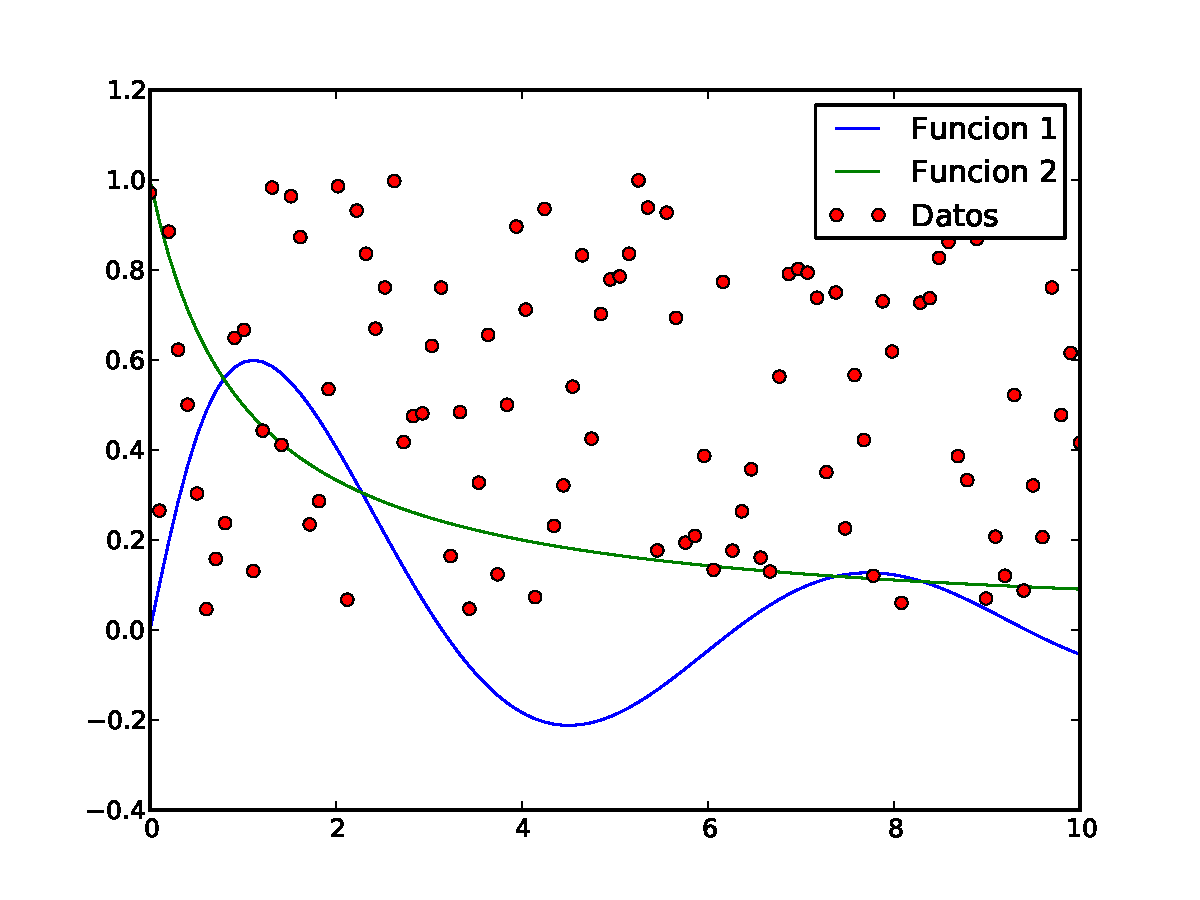
\includegraphics[width=0.7\textwidth]
	{./pictures/usage_01.pdf}

	\caption{\small{Resultado del ejemplo anterior, gráfica de dos funciones
	y datos aleatorios.}}
	
	\label{fig:small_pedulum}
\end{figure}
%.........................................................................


Para obtener el anterior script, el estudiante puede transcribirlo 
directamente de esta guía o puede descargarlo del repositorio oficial del 
curso\footnote{Repositorio oficial en 
\url{https://github.com/sbustamante/Computacional-Campos}} en el link
\url{https://github.com/sbustamante/Computacional-Campos/raw/master/codigos/usage\_01.py}.
Una vez obtenido el archivo \texttt{usage\_01.py}, abrir una terminal en la 
carpeta donde se ha guardado y escribir \texttt{ipython} para abrir el 
intérprete de \python


%.........................................................................
%Opening iPython
\begin{listing}[style=consola, numbers=none]
\$ ipython
\end{listing}
%.........................................................................


Se debe obtener algo como


%.........................................................................
%iPython
\begin{listing}[style=consola, numbers=none]
\$ ipython
Python 2.6.5 (r265:79063, Apr 16 2010, 13:57:41) 
Type "copyright", "credits" or "license" for more information.

IPython 0.10 -- An enhanced Interactive Python.
?         -> Introduction and overview of IPython's features.
%quickref -> Quick reference.
help      -> Python's own help system.
object?   -> Details about 'object'. ?object also works, ?? prints more.

In [1]: 
\end{listing}
%.........................................................................


Finalmente para ejecutar el script, usar el comando \texttt{run} seguido
del nombre del código en el intérprete de código \python


%.........................................................................
%Runing a script
\begin{listing}[style=consola, numbers=none]
In [1]: run usage_01.py
\end{listing}
%.........................................................................




%*************************************************************************

%#########################################################################



%#########################################################################
%	1. ELECTROSTATIC
%#########################################################################

%#########################################################################
\chapter{Electrostática}
\label{cha:electrostatic}

La electrostática estudia la interacción entre cuerpos cargados 
eléctricamente sin tener en cuenta su movimiento. Esta simplificación 
permite ignorar términos dinámicos asociados a corrientes eléctricas y 
campos magnéticos inducidos.

\

En este capítulo se realizan algunas demostraciones computacionales que 
van desde el cálculo de trayectorias de partículas en campos eléctricos y 
magnéticos, la representación de las líneas de campo y superficies 
equipotenciales de distribuciones de carga, hasta el cálculo de 
capacitancia de algunos sistemas.
%#########################################################################



\
%*************************************************************************
\section{Demostración 1: Espectrómetro de Masas}
\label{sec:DEMO2_01}
\rule{14cm}{0.5mm}

En esta primera demostración será estudiado el espectrómetro de masas. El 
objetivo de este dispositivo es caracterizar partículas cargadas de acuerdo
a su relación carga masa $(q/m)$. Su funcionamiento consiste en la inmersión 
de las partículas en un campo magnético o eléctrico (este caso) y a partir de
las trayectorias obtenidas determinar su relación carga masa (ver figura 
\ref{fig:mass_spectrometer}).

\

Tomando una partícula de masa $m$ y carga $q$ embebida en un campo eléctrico
homogéneo y uniforme $\bds E$, la ecuación de movimiento es


%.........................................................................
%Movement equation
\eq{eq:charged_particle}
{m\dtot{^2\bds r}{t^2} = q\bds E}
%.........................................................................


Tomando el sistema coordenado de tal forma que el campo $\bds E$ esté en la
dirección positiva de y, se obtiene


%.........................................................................
%Mass Spectrometer
\begin{figure}[htbp]
	\centering
	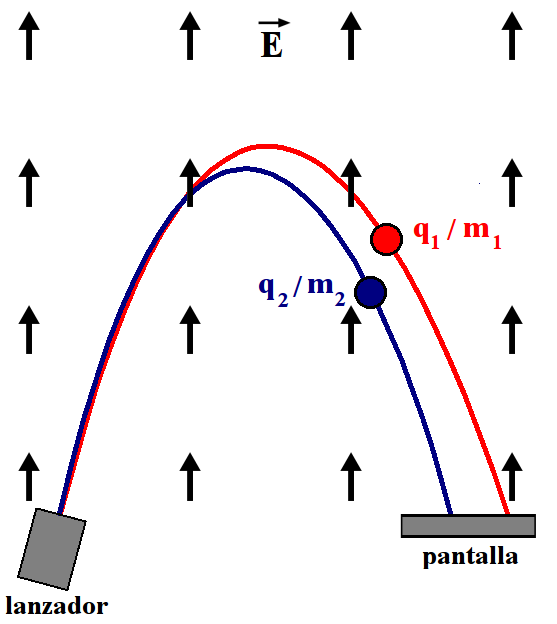
\includegraphics[width=0.50\textwidth]
	{./pictures/mass_spectrometer.png}

	\caption{\small{Espectrómetro de masas.}}
	
	\label{fig:mass_spectrometer}
\end{figure}
%.........................................................................


%.........................................................................
%Movement equations solution
\begin{eqnarray}
\label{eq:x_equation}
x(t) &=& x_0 + v_{x0}t \\
\label{eq:y_equation}
y(t) &=& y_0 + v_{y0}t + \frac{1}{2}\pr{\frac{q}{m}}t^2
\end{eqnarray}
%.........................................................................
donde se ha introducido la posición inicial de la partícula $\bds r(t=0) = 
(x_0, y_0)$ y la velocidad inicial $\bds v(t=0) = (v_{x0}, v_{y0})$.

\

Eliminando el tiempo de las dos ecuaciones se obtiene la siguiente 
trayectoria


%.........................................................................
%Trayectory
\eq{eq:trayectory}
{y(x) = y_0 + \frac{v_{y0}}{v_{x0}}(x - x_0) + 
\frac{1}{2}\pr{\frac{q}{m}} \pr{ \frac{x - x_0}{v_{x0}} }^2}
%.........................................................................

\

En el siguiente código de \python se grafica la trayectoria de dos 
partículas con diferente relación carga masa. La primera tiene una 
relación $q_1/m_1 = -1\mbox{ C}/1 \mbox{ kg}$ y la segunda $q_2/m_2 = 
-1\mbox{ C}/2 \mbox{ kg}$. Ambas partículas se disparan del origen y con 
una elocidad inicial de $\bds v_0 = (1, 2) \mbox{ m/s}$. El campo eléctrico 
tiene una intensidad de $|\bds E| = 1 \mbox{ N/C}$.

\newpage
%ccccccccccccccccccccccccccccccccccccccccccccccccccccccccccccccccccccccccc
%DEMO 2_01
\begin{listing}[style=python]
#!/usr/bin/env python
#==========================================================
# DEMOSTRACION 1
# Espectrometro de masas
#==========================================================
from __future__ import division
import numpy as np
import matplotlib.pylab as plt

#Trayectoria
def trayectory(x):
    y = y0 + vy0/vx0*(x - x0) + 0.5*(q/m)*( (x-x0)/vx0 )**2
    return y
    
#PARTICULA 1
#Carga
q = -1
#Masa
m = 1
#Posicion inicial
x0 = 0
y0 = 0
#Velocidad inicial
vx0 = 1
vy0 = 2
#Valores de X a graficar
X = np.arange( 0, 10, 0.01 )
#Trayectoria
Y = trayectory( X )
#Grafica de trayectoria
plt.plot( X, Y, label='particula 1' )

#PARTICULA 2
#Carga
q = -1
#Masa
m = 2
#Posicion inicial
x0 = 0
y0 = 0
#Velocidad inicial
vx0 = 1
vy0 = 2
#Valores de X a graficar
X = np.arange( 0, 10, 0.01 )
#Trayectoria
Y = trayectory( X )
#Grafica de trayectoria
plt.plot( X, Y, label='particula 2' )

#Limites del eje X
plt.xlim( (0,10) )
#Limites del eje Y
plt.ylim( (0,10) )
plt.legend()
plt.show()
\end{listing}
%ccccccccccccccccccccccccccccccccccccccccccccccccccccccccccccccccccccccccc


El resultado que se obtiene es


%.........................................................................
%Trayectories
\begin{figure}[htbp]
	\centering
	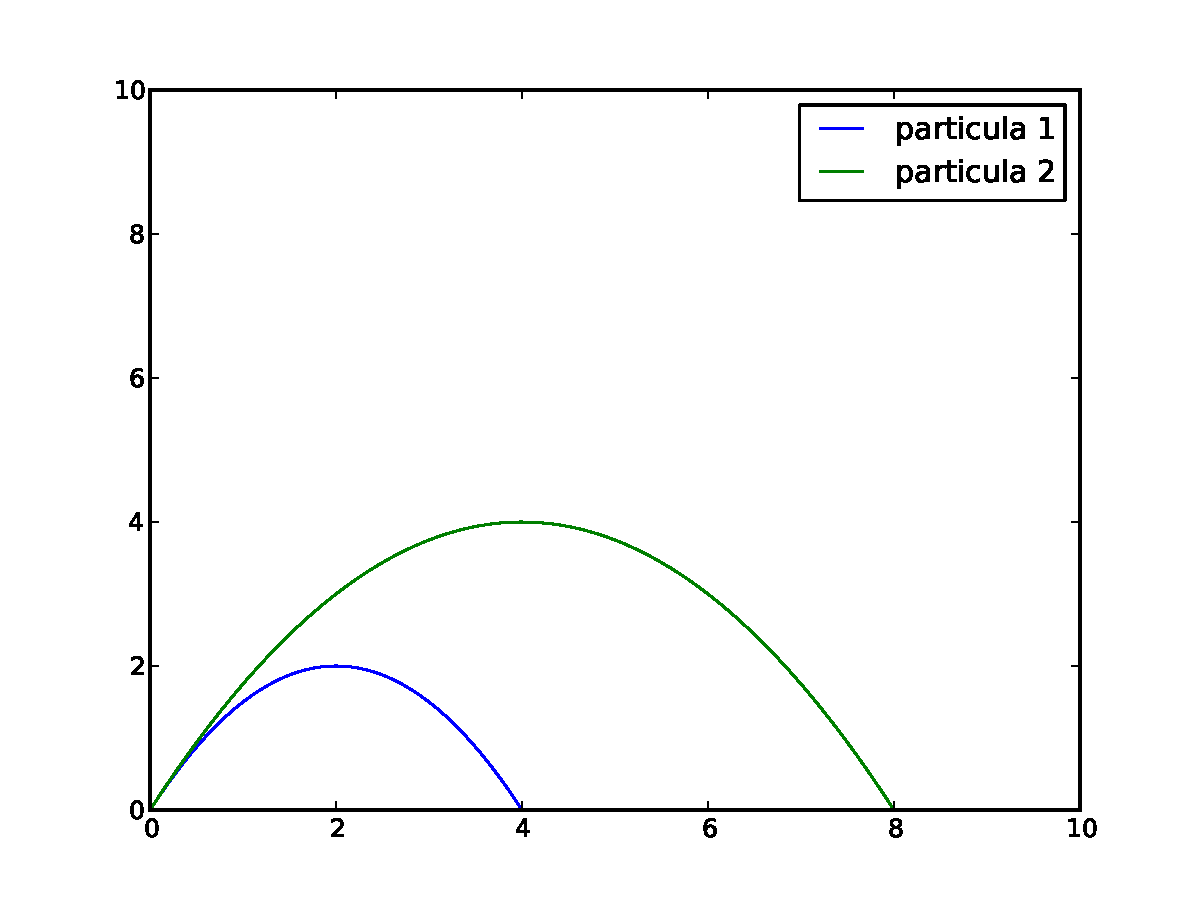
\includegraphics[width=0.8\textwidth]
	{./pictures/demo2_01.pdf}

	\caption{\small{Trayectorias según la relación carga masa de las 
	partículas.}}
	
	\label{fig:trayectories}
\end{figure}
%.........................................................................


La representación de la trayectoria de forma gráfica permite entonces 
comparar directamente con datos medidos en un laboratorio, por ejemplo 
trayectorias de partículas en cámaras de burbujas.

\newpage

A continuación se explica cada componente del código anterior


%ccccccccccccccccccccccccccccccccccccccccccccccccccccccccccccccccccccccccc
%DEMO 2_01
\begin{listing}[style=python, numbers = none]
from __future__ import division
import numpy as np
import matplotlib.pylab as plt
\end{listing}
%ccccccccccccccccccccccccccccccccccccccccccccccccccccccccccccccccccccccccc
En la primera línea se carga el módulo \texttt{division}, este permite a 
\python calcular fracciones de números enteros como cantidades reales. En
la siguiente línea se carga la librería \numpy con el alias de \texttt{np}
y finalmente se carga la librería \matplotlib con el alias de \texttt{plt}.


%ccccccccccccccccccccccccccccccccccccccccccccccccccccccccccccccccccccccccc
%DEMO 2_01
\begin{listing}[style=python, numbers = none]
#Trayectoria
def trayectory(x):
    y = y0 + vy0/vx0*(x - x0) + 0.5*(q/m)*( (x-x0)/vx0 )**2
    return y
\end{listing}
%ccccccccccccccccccccccccccccccccccccccccccccccccccccccccccccccccccccccccc
En esta parte se define la trayectoria de la partícula en el campo 
eléctrico descrito.

%ccccccccccccccccccccccccccccccccccccccccccccccccccccccccccccccccccccccccc
%DEMO 2_01
\begin{listing}[style=python, numbers = none]    
#PARTICULA 1
#Carga
q = -1
#Masa
m = 1
#Posicion inicial
x0 = 0
y0 = 0
#Velocidad inicial
vx0 = 1
vy0 = 2
#Valores de X a graficar
X = np.arange( 0, 10, 0.01 )
#Trayectoria
Y = trayectory( X )
#Grafica de trayectoria
plt.plot( X, Y, label='particula 1' )
\end{listing}
%ccccccccccccccccccccccccccccccccccccccccccccccccccccccccccccccccccccccccc
Se definen las propiedades físicas y cinemáticas de la partícula 1. Su 
carga, su masa, su posición y velocidad inicial. Luego, usando el comando
\texttt{arange} de la librería \numpy, se construye un arreglo de valores 
en el eje X que serán usados para el cálculo de la trayectoria. En este 
caso se toma desde 0 a $10$ m con un salto de $0.01$ m. Finalmente se 
llama la función de la trayectoria de la partícula en todos los valores de
\texttt{X} y se grafica, usando como etiqueta \texttt{label='particula 1'}.


%ccccccccccccccccccccccccccccccccccccccccccccccccccccccccccccccccccccccccc
%DEMO 2_01
\begin{listing}[style=python, numbers = none]
#Limites del eje X
plt.xlim( (0,10) )
#Limites del eje Y
plt.ylim( (0,10) )
plt.legend()
plt.show()
\end{listing}
%ccccccccccccccccccccccccccccccccccccccccccccccccccccccccccccccccccccccccc
Finalmente se usan las funciones de \matplotlib \texttt{xlim} y \texttt{ylim}
para fijar los límites de la ventana de graficación. La función 
\texttt{legend} muestra las etiquetas de las dos trayectorias y finalmente
\texttt{show} muestra en pantalla el resultado.


\rule{14cm}{0.5mm}
%*************************************************************************

%#########################################################################


\begin{thebibliography}{}
\bibitem[1]{purcell} Purcell E. M. Electricity and Magnetism, Berkeley 
Physics Course Vol. 2. Mc Graw Hill. 1965. 
\bibitem[2]{finn} Alonso \& Finn. Física, Campos y Ondas Vol. 2. Addison-Wesley. 
1998.
\bibitem[3]{sears} Sears, Zemanski, Young \& Freedman, Física Universitaria Vol. 2. 
Pearson Addison-Wesley, 11 ed, 2004.
\end{thebibliography}

\end{document}